%%%%%%%%%%%%%%%%%%%%%%%%%%%%%%%%%%%%%
%\chapter{Short term quantum computing}
\chapter{Noisy Intermediate-Scale Quantum (NISQ) Algorithms} % algorithms or computing?
% I like algorithms, it's more specific.
\label{chpt:shortqcomp}

% \epigraph{\textit{Let's put the short term section last}}{Andres}



\epigraph{\vspace{-1.5cm}\textit{Attaining quantum supremacy and exploring its consequences will be among the great challenges facing 21st century science, and our imaginations are poorly equipped to envision the scientific rewards of manipulating highly entangled quantum states, or the potential benefits of advanced quantum technologies.}}{John Preskill \cite{Preskill2012}} % As we rise to the call of the entanglement frontier, we should expect the unexpected.

% In this section we aim to give a comprehensive overview of quantum computing platforms which are currently available (only superconducting qubits) and discuss the near-term advantages that these platforms can bring.

% Intro NISQ algorithms chapter
% Q algorithms
% FTLSQ & NISQ
% Implementation in hardware
% Q supremacy
% nisq algorithms
% In this chapter...

\addcontentsline{toc}{section}{4.0 \hspace{0.3cm}Introduction}

% q algorithms
Quantum algorithms were first devised by David Deutsch in 1985 with the proposal of what nowadays is known as Deutsch's algorithm \cite{Deutsch1985}. The development of quantum algorithms exploded during the nineties with the proposal of several other quantum algorithms \cite{AM2016, zoo} as the famous Shor's and Grover's algorithms. Althought the problems addressed by quantum algorithms can be \emph{simulated} by classical computers, they cannot be \emph{efficiently simulated}, as in classical computers would require ridiculously long periods of time to do so. The appealing feature of quantum algorithms is that for particular types of problems, they offer speedups in comparison with their classical counterparts. 

% Many of these problems are specific abstract problems with interest from science, but there are some that will have a huge impact on society like Shor's and simulating chemistry for the development of drugs. Active area of research to find new algorithms, or to adapt existing ones to solve useful problems.

% FTLSQ, connecting with hardware, NISQ description
The great majority of quantum algorithms (if not all) were initially developed to be of a practical use when implemented in a Fault-Tolerant Large-Scale Quantum (FTLSQ) computer. A \emph{fault-tolerant} quantum device refers to a device having low enough noise such that is able to implement an algorithm with a decent \textcolor{blue}{(number?)} circuit depth. A \emph{large-scale} quantum device refers to a device being able to control a number of $\sim 10^6$ physical qubits \textcolor{blue}{(how many logical?)}. Even though the construction of FTLSQ devices is a long-term goal which is believed to be at least several decades away \cite{JLOqc2010}, it has recently entered to the so-called era of: Noisy Intermediate-Scale Quantum (NISQ) devices. A quantum device is considered \emph{noisy} when is able to implement quantum algorithms with a circuit depth of less than $1000$ gates. A \emph{intermediate-scale} quantum device refers to a device controlling a number of $\sim 50-100$ physical qubits \cite{Preskill2018}. Smaller devices $< 20$ have also been called \emph{quantum processors} \cite{Qiang2018}. % and therefore only small instances of the algorithms have been implemented in these small devices

% Implementation of algorithms in real hardware
Quantum algorithms are expected to outperform their classical counterparts when implemented in FTLSQ computers and they are not expected (in principle) to do so when implemented in quantum processors or NISQ devices. In fact, even though several of these quantum algorithms have already been implemented in quantum processors and NISQ devices, \emph{all} of these instances can be simulated by classical computers. In order to achieve the breaking point of having quantum devices that can efficiently run an algorithm which cannot efficiently be classically simulated, we need to keep further scaling up current quantum hardware and particularly, keep developing algorithms suitable to be run on NISQ devices. This breaking point has been coined as \emph{quantum supremacy}\footnote{In regards of the use of the term "Quantum Supremacy", we would like to quote Ref \cite{Road2017}:\\ \emph{The use of the word “supremacy”—which denotes “the state or condition of being superior to all others in authority”—was criticised in \cite{Road52107} because the syntagm ‘white supremacy’ is associated with the racial segregation and discrimination of the apartheid regime of South Africa. Proposals like “quantum advantage” or “quantum superiority” have been discussed \cite{Road42017}, but to date none has gained ground.}}. 
% with two characteristics in mind useful for the short-term and/or milestone. 

% The first quantum algorithm implemented was Shor's algorithm \cite{MatthewsShor}, the first quantum walk in IQP \cite{MatthewsWalks, Qiang2016}, the first Fermionic simulation in IQP \cite{MatthewsFermionic}, general mixed one-qubit states and violation of Bell inequalities \cite{Shadbolt2011a}, simulating quantum chemistry \cite{Peruzzo2014}, quantum complexity \cite{Carolan2014}, delayed choice experiment \cite{Shadbolt2014} and very recently Deutsch's and Gedik's algorithms \cite{Qiang2018}.

% \footnote{issue about supremacy (and ancilla) Weisner}

% q supremacy
Quantum supremacy refers to the implementation of a quantum algorithm that cannot be efficiently implemented in a classical computer. Achieving quantum supremacy is a milestone for quantum computing which has not been reached yet, and it is a very active area of research. The term was first introduced by Preskill in \cite{Preskill2012} and further formalised later by Harrow and Montanaro \cite{HarrowMontanaro2017}. Quantum supremacy through Boson sampling seems rather further away from what was expected \cite{QAdvantage} and theoretical works predict a minimum amount of $~90$ qubits in order to achieve it \cite{Harrow2018}. In \autoref{fig:NISQ} we have the research direction taken by Google in terms of quantum computing, specifying: NISQ era, FTLSQ era and the breaking point of quantum supremacy. It is fair to say that this is the general trend that most companies working on quantum computing are currently following.

\begin{figure}[h!]
    \centering
    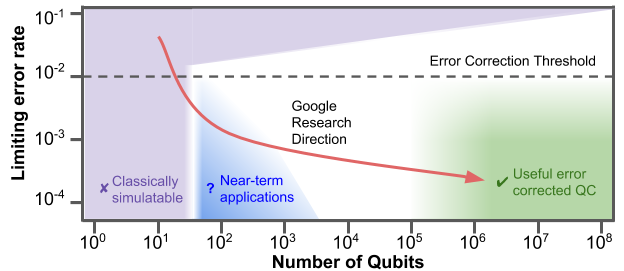
\includegraphics[scale=0.6]{figures/NISQ.png}
    \caption{Google quantum computing research direction. Quantum devices with $~50$ or less qubits can be simulated with classical computers. NISQ devices are being considered as those with $50-100$ qubits. Near-term devices are those containing from $50$ to a few thousands qubits. FTLSQ devices will contain $10^5$ qubits. Quantum supremacy refers to an implementation that cannot be classically simulated. Image taken from \cite{NISQ}.}
    \label{fig:NISQ}
\end{figure}

% Algorithms for nisq devices (whether useful now or for supremacy)
There are several candidates algorithms in the race for quantum supremacy and a not comprehensive list includes the following: Quantum optimisers such as the Quantum Approximate Optimisation Algorithm (QAOA) \cite{QAOA1,QAOA2,QAOA3} particularly the Variational Quantum Eigensolver (VQE) \cite{ES1,ES2}, adiabatic quantum computing such as quantum annealing \cite{AQC}, quantum deep and machine learning \cite{QML1,QML2}, quantum matrix inversion \cite{QMatrixInversion}, quantum recommendation systems \cite{QRecommendation}, quantum semidefinite programming (QSDP) \cite{QSDP1,QSDP2}, quantum simulation \cite{QS1}, quantum games \cite{JW2018}, and quantum kitchen sinks \cite{QKitchenSinks2018}. In this chapter we are going to address some basic examples for quantum annealing and the variational quantum eigensolver (VQE).  % Q annealing reasons? there's alot of controversy but could be useful. VQE Reasons? VQE cool for chemists, perhaps a good candidate for Q supremacy or Q advantage? and caviate here is we are addressing these algorithms as for the near-term but they all can achieve full potential in long term.

% QAOA is  (max cut)

% to give a taste of both cases useful and possibly useful for QS.

% In Chapter 1 qm background where we addressed the fundamentals, chapter 2 into to different Q software available, chapter 3 analytical description of algorithms. Now In chapter 4 we address two particular examples of the algorithms that are very likely to be implemented in the short-term, namely dwave stuff and quantum variational eigensolver (QVE).

% Quantum computing was first devised in the early eighties by Richard Feynman when considering the possibility of simulating complex quantum physical systems using another quantum physical system \cite{Feynman1982}, 

% A machine capable of implementing these quantum algorithms has been coined an \emph{universal quantum computer} \cite{JLOqc2010} (or general purpose), and its construction has become one of the main goals (if not the holy grail) of this ongoing second quantum revolution.

%%%%%%%%%%%%%%
\begin{comment}
Paragraph on short term
\begin{itemize}
    \item Q Supremacy first time defined \cite{Preskill2012}
    \item NISQ era defined \cite{Preskill2018}
    \item Q advantage/supremacy \cite{QAdvantage}
    \item theoretical work on the amount of qubits needed for it \cite{Harrow2018}, 
    \item the article suggesting supremacy with Boson sampling is far away \cite{QAdvantage}.
\end{itemize}
\end{comment}
%%%%%%%%%%%%%%
%%%%%%%%%%%%%%
\begin{comment}
(one-ref each). JP classification.
\begin{itemize}
\item 
    \begin{itemize}
        \item eigensolver \cite{ES1,ES2,ES3,ES4,ES5,ES6,ES7}
        \item 
    \end{itemize}
\item Q annealing \cite{AQC}
\item Q deep (machine) learning \cite{QML1,QML2}
\item Q matrix invertion \cite{QMatrixInversion}
\item Q recommendation systems \cite{QRecommendation}
\item Q SDP \cite{QSDP1,QSDP2}
\item Q simulation (digital and analogue) \cite{QS1} %anthony laing stuff?
\item Q games \cite{JW2018} %JP doesnt cite Wooton but we are gonna do it
\end{itemize}
    
Other Q algorithms/tasks not covered by JP
\begin{itemize}   
\item Boson sampling? inside simulation? Reference stating that it;s gonna take quite a bit for supremacy \cite{QAdvantage}.
\item kitchen sinks \cite{QKitchenSinks2018}
\item anything else? 
\end{itemize}
\end{comment}
%%%%%%%%%%%%%


% Jake
%Im not sure yet if this is the only section on quantum annealers but if it is maybe we want to add more of a discussion after the examples of my this is a short term limited technology? (If it is, I do remember someone saying to me that it could be universal but Im not sure I agree with that)

%%%%%%%%%%%%%%%%
\section{Adiabatic quantum computing \& quantum annealers}
%%%%%%%%%%%%%%%%%%%%%%%%%%%%%%%%%%%%
%%%%%%%%%%%%%%%%%%%%%%%%%%%%%%%%%%%%
%%%%%%%%%%%%%%%%%%%%%%%%%%%%%%%%%%%%
%%%%%%%%%%%%%%%%%%%%%%%%%%%%%%%%%%%%


 
In this section, we will present the example of vertex coloring problem using both D-Wave ocean stack as well as 1QBIT QUANTUM-READY™ SDK following the algorithm discussed in the section \ref{sec:annealing}.


%%%%%%%%%%%%%%%%%%%%%%%%%%%%%%%%%%%%%%%%%%
\subsection{Vertex Coloring with 1QBIT QUANTUM-READY™ SDK }
\begin{tcolorbox}[standard jigsaw,
    opacityback=0,  % this works only in combination with the key "standard jigsaw"
    boxrule=0.5pt,label={vertexcoloring}]
    {\bf Example: Vertex Coloring}
    \tcbline 
    Let’s solve the vertex coloring problem for the configuration shown in Figure \ref{fig:graph}
\end{tcolorbox}
\begin{figure}[h!]
\caption{Problem setting and sample solution of vertex coloring problem}
    \centering
    \begin{subfigure}[b]{0.4\textwidth}
        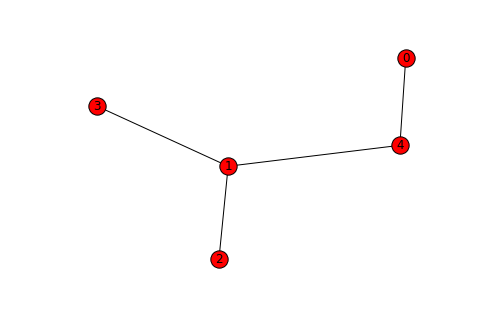
\includegraphics[width=\textwidth]{graph.png}
        \caption{Problem setting of the Vertex Coloring}
        \label{fig:graph}
    \end{subfigure}
     \begin{subfigure}[b]{0.4\textwidth}
        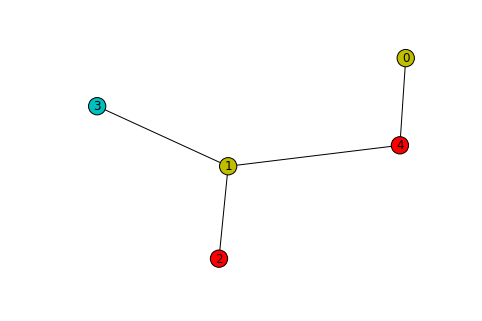
\includegraphics[width=\textwidth]{figures/colored.png}
        \caption{Final configuration after coloring}
        \label{fig:coloured}
    \end{subfigure}
\end{figure}
First we want to import the \texttt{networkx} and \texttt{matplotlib} library for the graph plotting.   
\begin{minted}{python}
import networkx as nx 
import matplotlib.pyplot as plt 

from qdk.binary_polynomial import * 
from qdk.common_solver_interface import * 
\end{minted}
The configuration of the coloring program is set by setting the nodes and neighbours.  The graph of the confifuration can be drawn.
\begin{minted}{python}
# Set the graph configuration by setting nodes and neighbours 
nodes = [0,1,2,3,4] 
neighbours = [(0,4),(1,2),(1,3),(1,4)] 
# Draw the graph configuration 
g = nx.Graph() 
g.add_nodes_from(nodes) 
g.add_edges_from(neighbours) 
pos = nx.spring_layout(g) 
nx.draw(g, pos=pos, with_labels=True, node_color='w', node_size=1000) 
plt.show() 
\end{minted}
As only one dimensional QUBO problem can be solved, the equation should be reduced to one dimension by reordering the index $n,k \rightarrow nK+k$.
\begin{minted}{python}
# Turn the two dimension index to one dimension
def d2tod1(n, k, K):  
    return n * K + k  
\end{minted}
Define the function to transfer the final solution to the colour label on the graph.
\begin{minted}{python}
# Function to color the final configuration
pallete = {0: 'r', 1: 'c', 2:'m', 3:'y'} 
def get_color(n, sol, K): 
    z = d2tod1(n, 0, K) 
    color = 0 
    for k in range(K): 
        if sol[z + k]: 
            break 
     return pallete[k] 
\end{minted}
Build the quadratic equation for vertex colouring problem:
\begin{equation}
H = \sum_{n=0}^{N-1}(1-\sum_{k=0}^{K-1}x_{nK+k})^2 + \sum_{(u,v)\in E}\sum_{k=0}^{K-1}x_{uK+k}x_{vK+k}
\end{equation}
\begin{minted}{python}
# Construct the quadratic equation 
builder = QuadraticBinaryPolynomialBuilder() 
qubo = builder.build_polynomial() 
N = 5 
K = 4
for n in range(N):
    builder.add_constant_term(1)
    for k in range(K):
        builder.add_term(-1, d2tod1(n,k,K))
    builder.power(2)
    t = builder.build_polynomial()
    qubo.sum(t)
    builder.reset()

for (u,v) in g.edges():
    for k in range(K): 
        builder.add_term(1, d2tod1(u,k,K), d2tod1(v,k,K))
        qubo.sum(builder.build_polynomial())
print (qubo) 
\end{minted}
We then set up the local solver and sample for 300 times
\begin{minted}{python}
solver = DWaveSolver() 
solver.solver.num_reads = 300 
sol = solver.minimize(qubo).peek_minimum_energy_solution().configuration 
\end{minted}
Finally we can draw the final configuration using the node\_color function defined.
\begin{minted}{python}
# Draw the final configuration with color applied
nx.draw(g, pos=pos, with_labels=True, nodelist=g.nodes(),  
node_color=[get_color(n, sol, K) for n in g.nodes()], node_size=1000) 
plt.show() 
\end{minted}

\begin{comment}
\inputminted{python}{code/dwave/colouring_qdk.txt}
\end{comment}

%%%%%%%%%%%%%%%%%%%%%%%%%%%%%%%%%%%%%%%%%
\subsection{Vertex Colouring with Ocean}
Following really similar steps, the same colouring problem can be implemented on D-Wave Ocean.

\inputminted{python}{code/dwave/colouring_ocean.txt}
%%%%%%%%%%%%%%%%%%



%%%%%%%%%%%%%%%%%%%%%%%%%%%%%%%%%%%%%%%%%%
%%%%%%%%%%%%%%%%%%%%%%%%%%%%%%%%%%%%%%%%%%
%%%%%%%%%%%%%%%%%%%%%%%%%%%%%%%%%%%%%%%%%%
%%%%%%%%%%%%%%%%%%%%%%%%%%%%%%%%%%%%%%%%%%
\section{Implementation of the Variational Quantum Eigensolver (VQE) Algorithm}
%%%%%%%%%%%%%%%%%%%%%%%%%%%%%%%%%%%%%%%%%%
%%%%%%%%%%%%%%%%%%%%%%%%%%%%%%%%%%%%%%%%%%
%%%%%%%%%%%%%%%%%%%%%%%%%%%%%%%%%%%%%%%%%%
%%%%%%%%%%%%%%%%%%%%%%%%%%%%%%%%%%%%%%%%%%

In this section we are going to implement a simple example of the VQE algorithm, using the libraries provided by pyQuil and QISKit. This algorithm can also be implemented in Project Q and Q\# but it needs to be done from scratch, so it is left as an exercise to the interested reader.

%%%%%%%%%%%%%%%%%%%%%%%%%%%%%%%%%%%
\subsection{VQE Algorithm in pyQuil}
%%%%%%%%%%%%%%%%%%%%%%%%%%%%%%%%%%%%

In this subsection we are going to use the VQE algorithm from Grove's library to address the following simple VQE problem.

%%%%%%%%%%%% title= Example 1
\begin{tcolorbox}[standard jigsaw,
    opacityback=0,  % this works only in combination with the key "standard jigsaw"
    boxrule=0.5pt,label={example0000001}]
    {\bf Example: A simple VQE algorithm in pyQuil}
    \tcbline
    Consider the one-qubit Hamiltonian $H=\sigma_z$  and an ansatz given by:
    $\ket{\psi\left(\theta\right)}=\cos{\theta/2}\ket{0}-i\sin{\theta/2}\ket{1}={\rm RX}(\theta)\ket{0}$.
    \begin{comment}
    \begin{align*}
    H=\sigma_z,
    \end{align*}
    and an ansatz given by:
    \begin{align*}
    \ket{\psi\left(\theta\right)}=\cos{\theta/2}\ket{0}-i\sin{\theta/2}\ket{1}={\rm RX}(\theta)\ket{0}.
    \end{align*}
    \end{comment}
    Find the ground state energy of the system.
\end{tcolorbox}
%%%%%%%%%%%%%%%

Spoiler alert, this Hamiltonian has eigenvalues $+1,-1$, so the ground state energy is $-1$ which corresponds to the eigenvector $\ket{\psi(\theta=\pi)}=i\ket{1}$. However, we now want a quantum computer to do this by sampling different Ansatzes. This is interesting because for huge matrices, this VQE does better than classical methods at finding the ground eigenvalue.

\begin{minted}{python}
# 1. Calling Libraries
from pyquil.quil   import Program
from pyquil.api    import QVMConnection
from pyquil.gates  import RX
from pyquil.paulis import sZ,PauliSum,PauliTerm

# Calling Grove Library and optimiser
from grove.pyvqe.vqe import VQE 
import numpy as np
from scipy.optimize  import minimize

# 2. Initialising
qp = Program()
qvm = QVMConnection()
vqe = VQE(minimizer=minimize, minimizer_kwargs={'method': 'nelder-mead'})

# 3. Defining ansatz
def ansatzv(theta): # input vectors. 
    qp1 = Program()
    qp1.inst(RX(theta[0],0))
    return qp1
    
# 4. Defining Hamiltonian
hamiltonian = sZ(0) 

# 5. Running the VQE
initial_angle = [0.0]
result = vqe.vqe_run(ansatzv, hamiltonian, initial_angle, None, qvm=qvm) 
print(result)
\end{minted}

\begin{enumerate}
    \item \textbf{Calling libraries} - We start by stating the libraries that we are going to use, quil, api, gates and now we also need paulis. We also need to call the vqe from grove and minimize from scipy.
    \item \textbf{Initialising} - We initialise an object program, the connection to the QVM and a vqe object, setting the classical optimiser as being the Nelder Mead.
    \item \textbf{Defining the Ansatz} - In pyQuil we are allowed to address the Ansatz. In this case we are directly implementing the required Ansatz as program in terms of an input angle.
    \item \textbf{Defining Hamiltonian} - The Hamiltonian should be input as in terms of the pauli matrices and the paulis dictionary.
    \item \textbf{Running the VQE} - We run the VQE with inputs being the ansatz program, a vector with initial the initial angle and the Hamiltonian of interest.
\end{enumerate}

Printing results we first obtain the value of the parameter for which the minimum has been achieved, followed by the minimum.
\begin{minted}{python}
{'x': array([3.1415625]), 'fun': -0.9999999995453805}
\end{minted}
We are obtaining the expected answer as ground energy of $-1$ with ground state $\ket{\psi\left(\theta\right)}=\cos{\theta}\ket{0}-i\sin{\theta/2}\ket{1}={\rm RX}(\theta/2)\ket{0}$, with $\theta=\pi$.

%%%%%%%%%%%%%
%%%%%%%%%%%%%
\begin{comment}
%%%%%%%%%%%%%%%%%
\begin{lstlisting}[language=Python,caption={Example VQE algorithm implemented with pyQuil (Grove).},label={lst:ExampleQVM},frame=single]
# Python Libraries
import numpy as np
from scipy.optimize  import minimize
# Calling pyQuil modules
from pyquil.quil   import Program
from pyquil.api    import QVMConnection
from pyquil.gates  import I,X,Y,Z,H,RX,RY,CNOT
from pyquil.paulis import sZ,PauliSum,PauliTerm
# Calling Grove Library
from grove.pyvqe.vqe import VQE 
# Defining Program object and renaming
qp=Program()
qvm=QVMConnection()
vqe=VQE(minimizer=minimize,minimizer_kwargs={'method': 'nelder-mead'})
# Defining ansatz
def ansatzv(theta): # input vectors. 
    qp1=Program()
    qp1.inst(RX(theta[0],0))
    return qp1
# Defining Hamiltonian
hamiltonian = sZ(0) 
initial_angle = [0.0]
# Running the VQE
result = vqe.vqe_run(ansatzv, hamiltonian, initial_angle, None, qvm=qvm) # VQE
print(result)
\end{lstlisting}
\end{comment}
%%%%%%%%%%%%%
%%%%%%%%%%%%%

%%%%%%%%%%%%%%
%%%%%%%%%%%%%%
\begin{comment}
%%%%%%%%%%%%%%%%%%%%%%%%%%%%%%%%%%%%%
\subsection{Step by step description}
%%%%%%%%%%%%%%%%%%%%%%%%%%%%%%%%%%%%%

Here I'm supposed to fully explain each step, in progress.

Calling Libraries and defining objects:
\begin{lstlisting}[language=Python,label={lst:ExampleQVM},frame=single]
# Python Libraries
import numpy as np
from scipy.optimize  import minimize
# Calling pyQuil modules
from pyquil.quil   import Program
from pyquil.api    import QVMConnection
from pyquil.gates  import I,X,Y,Z,H,RX,RY,CNOT
from pyquil.paulis import sZ,PauliSum,PauliTerm
# Calling Grove Library
from grove.pyvqe.vqe import VQE 
# Defining Program object and renaming
qp=Program()
qvm=QVMConnection()
vqe=VQE(minimizer=minimize,minimizer_kwargs={'method': 'nelder-mead'})
\end{lstlisting}

Defining our ansatz:
\begin{lstlisting}[language=Python,label={lst:ExampleQVM},frame=single]
# Defining ansatz
def ansatzv(theta): # input vectors. 
    qp1=Program()
    qp1.inst(RX(theta[0],0))
    return qp1
\end{lstlisting}    

Defining Hamiltonian.
\begin{lstlisting}[language=Python,label={lst:ExampleQVM},frame=single]
hamiltonian = sZ(0) 
\end{lstlisting}

Three levels:

{\bf 1.} Calculating the expectationv alue directly (this is cheating, but nice to make comparisons)
\begin{lstlisting}[language=Python,label={lst:ExampleQVM},frame=single]
result1=vqe.expectation(ansatz(theta1), hamiltonian, None, qvm)  # no sampling
print(result1)
\end{lstlisting}

{\bf 2.} Doing sampling
\begin{lstlisting}[language=Python,label={lst:ExampleQVM},frame=single]
result2=vqe.expectation(ansatz(theta1), hamiltonian, 10000, qvm) # sampling
print(result2)
\end{lstlisting}

{\bf 3.} Finally, the actual eigensolver
\begin{lstlisting}[language=Python,label={lst:ExampleQVM},frame=single]
result3=vqe.vqe_run(ansatzv, hamiltonian, initial_angle, None, qvm=qvm) # VQE
print(result3)
\end{lstlisting}
\end{comment}

%%%%%%%%%%%%%%%%%%%%%%%%%
\subsection{VQE algorithm in QISKit} % \color{blue}
%%%%%%%%%%%%%%%%%%%%%%%%%%%%%
Applications that can run on ibmqx4 include simulation of quantum state evolution and solving for the lowest energy of the system using a VQE. QISKit Aqua provides tools that can be used to make an eigensolver for the ground state energy of simple systems.

The first example we will explore is the case of finding the lowest eigenvalue for the $Z$ Pauli matrix. By inspection, we know that the value is $-1$. We can confirm that QISKit can also figure this out using the code seen in \autoref{aqua1}. The backend is specified as the local qasm simulator, which means this is being run on the local CPU. This initial step allows us to define our operator matrix in terms of the Paulis. The coefficients specify multipliers of these matrices. The next part details how we will run this code, and where it will be run (the backend). \texttt{algo\_input} represents the input of the code that is described by the operator made of Paulis in the pauli dictionary. The algorithm input is then further specified as the instance of the energy of the system, labelled as EnergyInput in the QISKit nomenclature. 

\begin{listing}[H]
\begin{minted}{python}
from qiskit_aqua import Operator, run_algorithm
from qiskit_aqua.input import get_input_instance
# Defines the dictionary of pauli operations
pauli_dict = {"paulis": [
    { "coeff": { "imag": 0.0, "real": 1.0 }, "label": "Z"}]}
algo_input = get_input_instance("EnergyInput")
algo_input.qubit_op = Operator.load_from_dict(pauli_dict)
params = {
  "algorithm": { "name": "VQE" },
  "optimizer": { "name": "SPSA" },
  "variational_form": { "name": "RY", "depth": 5 },
  "backend": { "name": "local_qasm_simulator" }}
# Runs a local simulation to produce the energy result
result = run_algorithm(params, algo_input)
print(result["energy"])
\end{minted}
\caption{The example code that uses the VQE to find the lowest eigenvalue of the $Z$ pauli operator. Code modified from the one that can be found at \cite{QISKitAqua}}
\label{aqua1}
\end{listing}

After a few minutes of running, this code produces the result of $-1.0$. This is exactly what we would expect to see.

The next example provided on the IBM QISKit Aqua site details a basic working code that displays the energy result of an operator that we can define in terms of tensor products of the Pauli matrices $X$ and $Z$, as seen in \autoref{eq:VQEIBM}. These matrices and their corresponding alpha coefficients specify an operator from which we can extract energy eigenvalues. This is labelled by the pauli dictionary in the code \autoref{aqua2}. Once again, the calculation is done on the local simulator. 

\begin{equation}
    O = \alpha_{1} \left(Z \otimes X\right) + \alpha_{2} \left(Z \otimes Z\right) + \alpha_{3} \left(X \otimes Z\right)
    \label{eq:VQEIBM}
\end{equation}

\begin{listing}[H]
\begin{minted}{python}
from qiskit_aqua import Operator, run_algorithm
from qiskit_aqua.input import get_input_instance
# Defines the dictionary of tensor products of pauli operations and the alpha coefficients we described in the operator equation
pauli_dict = {"paulis": [
    { "coeff": { "imag": 0.0, "real": 0.5 }, "label": "ZX" },
    { "coeff": { "imag": 0.0, "real": -1.0 }, "label": "ZZ" },
    { "coeff": { "imag": 0.0, "real": 0.5 }, "label": "XZ" }]}
algo_input = get_input_instance("EnergyInput")
algo_input.qubit_op = Operator.load_from_dict(pauli_dict)
# Defines the algorithm input in terms of the pauli dict and that we want the energy value
params = {
  "algorithm": { "name": "VQE" },
  "optimizer": { "name": "SPSA" },
  "variational_form": { "name": "RY", "depth": 5 },
  "backend": { "name": "local_qasm_simulator" }}
# Runs a local simulation in qasm to produce the energy result
result = run_algorithm(params, algo_input)
# Prints the final result of the energy of the system
print(result["energy"])
\end{minted}
\caption{The example code that utilises the VQE as presented in the QISKit Aqua documentation that prints the result of the energy of the system defined in it. Modified code originally found at \cite{QISKitAqua}.}
\label{aqua2}
\end{listing}

The result function is imported at the start from qiskit aqua and takes the parameters (params) dictionary that specifies the algorithm being run, the python optimizer (of which there are several) used and the backend used to run the code plus the two-qubit system defined by the pauli dict list as arguments. The results printed in the first three runs (and a few minutes of patiently waiting) of this code were: -1.4560546875, -1.4287109375 and -1.3896484375. All the decimal points have been kept to illustrate the slight changes that occur between iterations. This method is sensitive to the changes in the coefficients applied to the matrices used to define the operator. 

%%%%%%%%%%%%%%%%%%%%%%%%%%%%%%%%%%%%%%%%%
%\subsection{\color{red}TODO VQE algorithm in Project Q?}
%%%%%%%%%%%%%%%%%%%%%%%%%%%%%%%%%%%%%%%%%

% This would be quite nice, because According to Ryan LaRose's Guide, Microsoft does not have a function for this, so it'd be cool if our guide provides this, but of course Friki, only if there's enough time :3

%%%%%%%%%%%%%%%%%%%%%%%%%%%
\section{TODO Summary and Outlook}


%%%%%%%%%%%%%%%%%%%%%%%%%%%%%%%%%%%%
\section{TODO Exercises}

\textbf{Exercise 1 with QISKIT Aqua VQE}
\\
Try and modify the coefficients $\alpha_{1,2,3}$ in the VQE code and change their corresponding operators to the following: $Z\otimes I$, $I \otimes X$ and $X \otimes I$. How does this affect the output from the code? How much does each answer vary from the mean output value if you run the code multiple times? You can simplify the arithmetic by automating the process in your code if you'd like.
\\
\\
\textbf{Exercise 2 with QISKIT Aqua VQE}
\\
Can we simulate a molecule in QISKit? We can compose a simulation of the ground-state energy of the Helium hydride molecular ion (HeH$^{+}$) in the VQE by using the approximations described in . We can use the supplementary information of that publication to add the additional operators and their matching coefficients. After running the new code, you should find that your value(s) is twice the value computed in the publication. Why could this be?  

%%%%%%%%%%%%% Old Deusch algm
\begin{comment}
\begin{multicols}{2}
%%%%%%%%%%%%%%%%%%%%%%%%%%%%%%%%

%%%%%%%%%%%%%%%%%%%%%%%%%%%%%%%%
\subsection{Deutsch's Algorithm}
%%%%%%%%%%%%%%%%%%%%%%%%%%%%%%%%

%%%%%%%%%%%%%%%%
\begin{tcolorbox}[standard jigsaw,
    opacityback=0,  % this works only in combination with the key "standard jigsaw"
    boxrule=0.5pt]
    {\bf Deutsch's Algorithm}
    \tcbline
    Given a function $f:\{0,1\}^2\rightarrow \{0,1\}$ promised to be either balanced or constant. We initialise the system in the state $\ket{00}$, we need to implement the gates $H^{\otimes 2}$ and then $U_f$ and then $H^{\otimes 2}$ and then perform a measurement in the computational basis.
\end{tcolorbox}
%%%%%%%%%%%%%%%

%%%%%%%%%%%%%%%%%
\begin{lstlisting}[language=Python,caption={Deutsch's algorithm implemented in Python only},label={lst:DApython},frame=single] 
import numpy as np
# State initialisation
state0=np.array([[1],[0],[0],[0]]) 
# Gate Implementation
H=(1/np.sqrt(2))*np.array([[1,1],[1,-1]]) 
state1=np.dot(np.kron(H,H),state0)        
U=np.array([[-1,0,0,0],
            [0,1,0,0],
            [0,0,-1,0],
            [0,0,0,1]])
state2=np.dot(U,state1)
state3=np.dot(np.kron(H,H),state2)
# Measurement: defining basis
ket0=np.array([[1],[0]])
ket1=np.array([[0],[1]])
ket00=np.kron(ket0,ket0)
ket01=np.kron(ket0,ket1)
ket10=np.kron(ket1,ket0)
ket11=np.kron(ket1,ket1)
# Measurement: projectors P00,P01,P10,P11
P00=np.dot(ket00,ket00.T)
P01=np.dot(ket01,ket01.T)
P10=np.dot(ket10,ket10.T)
P11=np.dot(ket11,ket11.T)
# Probability of obtaining: 00,01,10,11
prob00=np.trace(np.dot(P00,np.dot(state3,np.conj(state3).T)))
prob01=np.trace(np.dot(P01,np.dot(state3,np.conj(state3).T)))
prob10=np.trace(np.dot(P10,np.dot(state3,np.conj(state3).T)))
prob11=np.trace(np.dot(P11,np.dot(state3,np.conj(state3).T)))
print(prob00,prob01,prob10,prob11)
\end{lstlisting}
%%%%%%%%%%%%%%%%
\columnbreak

Now implementing this with pyQuil. We first need to learn how to add our own gates.

%%%%%%%%%%%%%%%%%
\begin{lstlisting}[language=Python]
# Defining our own gates
Ufma=np.array([[-1,0,0,0],
               [0,1,0,0],
               [0,0,-1,0],
               [0,0,0,1]]); 
p.defgate("Uf",Ufma); 
p.inst(("Uf",0,1)); 
\end{lstlisting}
%%%%%%%%%%%%%%%%

In \autoref{lst:DAqvm}

%%%%%%%%%%%%%%%%%
\begin{lstlisting}[language=Python,caption={Deutsch's algorithm with pyQuil},label={lst:DAqvm},frame=single]
import numpy as np
from pyquil.quil import Program
from pyquil.api import QVMConnection 
from pyquil.gates import X,Z,Y,H,I 
# Invoking and renaming
qvm=QVMConnection()
p=Program() 
# Gate implementation
p.inst(H(0),H(1)) 
# Assuming the given function gives
Ufma=np.array([[-1,0,0,0],
               [0,1,0,0],
               [0,0,-1,0],
               [0,0,0,1]]);
# Adding matrix as a gate               
p.defgate("Uf",Ufma); 
# Applying new gate and Hadamards
p.inst(("Uf",0,1)); 
p.inst(H(0),H(1))
# Measurements
p.measure(0,0)
p.measure(1,1) 
# Running the program
cr=[] 
results=qvm.run(p,cr,4) 
print(results)
\end{lstlisting}
%%%%%%%%%%%%%%%%

%%%%%%%%%%%%%%%%
\begin{tcolorbox}[standard jigsaw,
    opacityback=0,  % this works only in combination with the key "standard jigsaw"
    boxrule=0.5pt]
    {\bf Exercise 2: Bernstein-Vazirani Algorithm}
    \tcbline
    As in DJ with $n=3$, and given a function $f$ that is a parity function. Checking that the code indeed identifies the parity function
\end{tcolorbox}

\end{multicols}
\end{comment}
%%%%%%%%%%%%%


%%%%%%%%%%%%%% Old Rigetti code added by Ben
\begin{comment}
Rigetti has created an environment called Forest, amongst its contributions is a python library called PyQuil. With PyQuil one can simulate up to 26 qubits on the Quantum Virtual Machine (QVM). An example code from \cite{rigetti} is detailed below with comments to assist the reader:
%%%%%%%%%%%%%%%%%%%%%%%%%%%%%%%%%%%
\begin{lstlisting}[language=Python,float=h]
from pyquil.quil import Program
from pyquil.gates import H, CNOT
from pyquil.api import SyncConnection
# construct a Bell State program
p = Program()
p.inst(H(0))
p.inst(CNOT(0, 1))
# run the program on a QVM
qvm = SyncConnection()
result = qvm.wavefunction(p) 
# produces the output wavefunction of the Bell state
\end{lstlisting}
Rigetti also offers access to a 19 qubit processor they call 19Q. This API 
%%%%%%%%%%%%%%%%%%%%%%%%%%%%%%%%%%%%%%%%%%%
\begin{lstlisting}[language=Python,float=h]
import numpy as np
 
def incmatrix(genl1,genl2):
    m = len(genl1)
    n = len(genl2)
    M = None #to become the incidence matrix
    VT = np.zeros((n*m,1), int)  #dummy variable
 
    #compute the bitwise xor matrix
    M1 = bitxormatrix(genl1)
    M2 = np.triu(bitxormatrix(genl2),1) 
 
    for i in range(m-1):
        for j in range(i+1, m):
            [r,c] = np.where(M2 == M1[i,j])
            for k in range(len(r)):
                VT[(i)*n + r[k]] = 1;
                VT[(i)*n + c[k]] = 1;
                VT[(j)*n + r[k]] = 1;
                VT[(j)*n + c[k]] = 1;
 
                if M is None:
                    M = np.copy(VT)
                else:
                    M = np.concatenate((M, VT), 1)
 
                VT = np.zeros((n*m,1), int)
 
    return M
\end{lstlisting}
\end{comment}
%%%%%%%%%%%%%